\documentclass{article}
\usepackage[papersize={17.6cm,5.7cm},margin=0pt]{geometry}
\usepackage{tikz}
\usepackage{newtxtext,newtxmath}
\pagestyle{empty}
\parindent=0pt

% x(budget) = (log10 b - 0.6) * 2.55 cm ; y(rate) = rate * 2.7 cm
\newcommand{\xA}{0.253}  % 5
\newcommand{\xB}{1.020}  % 10
\newcommand{\xC}{2.035}  % 25
\newcommand{\xD}{2.802}  % 50
\newcommand{\xE}{3.570}  % 100
\newcommand{\xF}{4.585}  % 250
\newcommand{\xG}{5.352}  % 500
\newcommand{\xH}{6.120}  % 1000
\newcommand{\xEND}{6.45}
\newcommand{\HT}{2.7}

\newcommand{\stepcurve}[3]{\draw[#1] (0,#3) -- (#2,#3) -- (#2,\HT) -- (\xEND,\HT);}
\newcommand{\flatzero}[2]{\draw[#1] (0,#2) -- (\xEND,#2);}

\newcommand{\panelframe}[1]{%
  \foreach \y in {0,1.35,2.7}
    \draw[gray!28,line width=0.35pt] (0,\y) -- (\xEND,\y);
  \foreach \x in {\xA,\xB,\xC,\xD,\xE,\xF,\xG,\xH}
    \draw[gray!20,line width=0.35pt] (\x,-0.08) -- (\x,2.85);
  \draw[line width=0.6pt] (0,-0.08) -- (0,2.85);
  \draw[line width=0.6pt] (0,-0.08) -- (\xEND,-0.08);
  \foreach \y/\l in {0/0,1.35/{0.5},2.7/{1.0}}
    \node[left,font=\small,inner sep=2.5pt] at (0,\y) {\l};
  \node[rotate=90,font=\small] at (-1.02,1.35) {witness-complete rate};
  \node[font=\small\bfseries,anchor=north west] at (0.02,3.36) {#1};
  \foreach \x/\l in {\xA/5,\xB/10,\xC/25,\xD/50,\xE/100,\xF/250,\xG/500,\xH/1000}
    \node[below,font=\small,inner sep=3pt] at (\x,-0.08) {\l};
  \node[font=\small] at (3.2,-0.80) {context budget $B$ (triples, log scale)};
}

\begin{document}
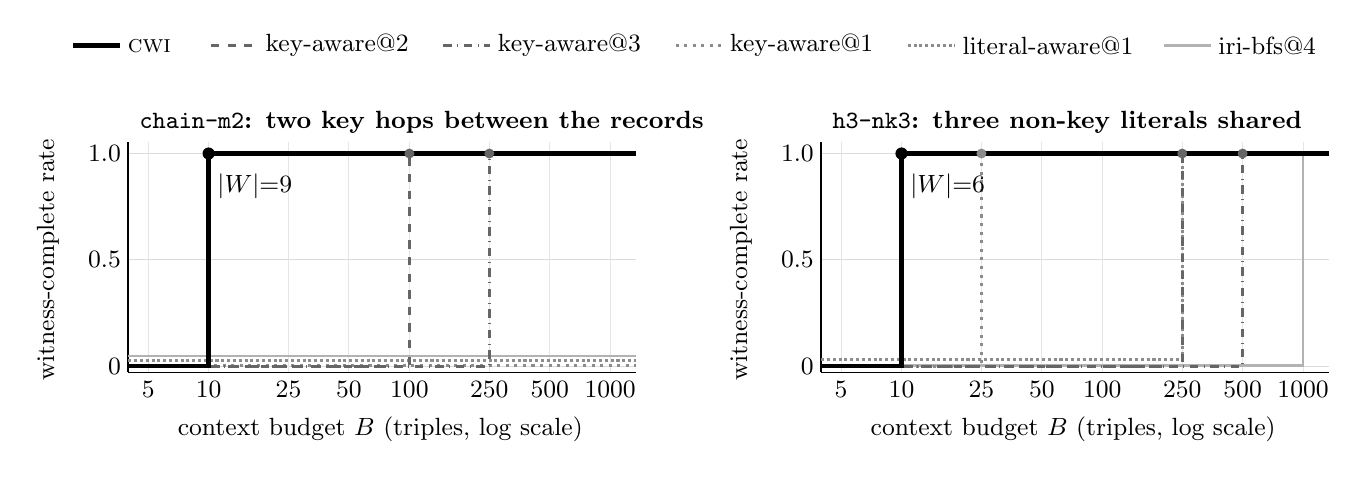
\begin{tikzpicture}[x=1cm,y=1cm]

%% ---------------- legend across the top ----------------
\begin{scope}[shift={(0.85,5.32)}]
  \draw[black,line width=1.7pt] (0,0) -- (0.6,0);
  \node[right,font=\small,inner sep=2.5pt] at (0.6,0) {\textsc{cwi}};
  \draw[black!60,dashed,line width=1.1pt] (1.75,0) -- (2.35,0);
  \node[right,font=\small,inner sep=2.5pt] at (2.35,0) {key-aware@2};
  \draw[black!60,dash dot,line width=1.1pt] (4.70,0) -- (5.30,0);
  \node[right,font=\small,inner sep=2.5pt] at (5.30,0) {key-aware@3};
  \draw[black!45,dotted,line width=1.1pt] (7.65,0) -- (8.25,0);
  \node[right,font=\small,inner sep=2.5pt] at (8.25,0) {key-aware@1};
  \draw[black!45,densely dotted,line width=1.1pt] (10.60,0) -- (11.20,0);
  \node[right,font=\small,inner sep=2.5pt] at (11.20,0) {literal-aware@1};
  \draw[black!30,line width=1.0pt] (13.85,0) -- (14.45,0);
  \node[right,font=\small,inner sep=2.5pt] at (14.45,0) {iri-bfs@4};
\end{scope}

%% ---------------- left panel: chain-m2 ----------------
\begin{scope}[shift={(1.55,1.25)}]
  \panelframe{\texttt{chain-m2}: two key hops between the records}
  \flatzero{black!30,line width=1.0pt}{0.13}
  \flatzero{black!45,densely dotted,line width=1.1pt}{0.070}
  \flatzero{black!45,dotted,line width=1.1pt}{0.012}
  \stepcurve{black!60,dash dot,line width=1.1pt}{\xF}{0}
  \stepcurve{black!60,dashed,line width=1.1pt}{\xE}{0}
  \stepcurve{black,line width=1.7pt}{\xB}{0}
  \fill[black]   (\xB,\HT) circle (2.2pt);
  \fill[black!60](\xE,\HT) circle (1.8pt);
  \fill[black!60](\xF,\HT) circle (1.8pt);
  \node[font=\small,anchor=west,inner sep=3pt] at (\xB,2.28) {$|W|{=}9$};
\end{scope}

%% ---------------- right panel: h3-nk3 ----------------
\begin{scope}[shift={(10.35,1.25)}]
  \panelframe{\texttt{h3-nk3}: three non-key literals shared}
  \stepcurve{black!30,line width=1.0pt}{\xH}{0.012}
  \stepcurve{black!45,dotted,line width=1.1pt}{\xC}{0}
  \stepcurve{black!45,densely dotted,line width=1.1pt}{\xF}{0.080}
  \stepcurve{black!60,dash dot,line width=1.1pt}{\xG}{0}
  \stepcurve{black!60,dashed,line width=1.1pt}{\xF}{0}
  \stepcurve{black,line width=1.7pt}{\xB}{0}
  \fill[black]   (\xB,\HT) circle (2.2pt);
  \fill[black!45](\xC,\HT) circle (1.8pt);
  \fill[black!60](\xF,\HT) circle (1.8pt);
  \fill[black!60](\xG,\HT) circle (1.8pt);
  \node[font=\small,anchor=west,inner sep=3pt] at (\xB,2.28) {$|W|{=}6$};
\end{scope}

\end{tikzpicture}
\end{document}
